\documentclass{article}
\usepackage{times}
\usepackage{graphicx}
\usepackage{subfigure}
\usepackage{natbib}
\usepackage{algorithm}
\usepackage{algorithmic}
\newcommand{\theHalgorithm}{\arabic{algorithm}}
\usepackage{hyperref}

\usepackage{mathtools}
\usepackage{amsmath}
\usepackage{amsthm}
\usepackage{amssymb}
\usepackage{cleveref}
\usepackage{cancel}

\usepackage{color}
\definecolor{darkgreen}{rgb}{0,.5,0}
\definecolor{mycyan}{rgb}{0,.9,.9}

\usepackage{tabularx}

\usepackage{tikz}

% Break in equations...
\allowdisplaybreaks

% Commonly used sets
\newcommand{\Z}{\mathbb{Z}}   % Integers
\newcommand{\R}{\mathbb{R}}   % Real numbers
\newcommand{\N}{\mathbb{N}}   % Natural numbers

% Symbols
\newcommand{\es}{\varnothing}  % Empty set
\newcommand{\e}{\varepsilon}   % Epsilon
\newcommand{\sub}{\subseteq}   % Subset
\renewcommand{\d}{\partial}    % Partial
\renewcommand{\th}{\theta}     % Theta
\renewcommand{\O}{\mathcal{O}} % Landau's symbol

% Operators
\renewcommand{\Re}{\operatorname{Re}}
\renewcommand{\Im}{\operatorname{Im}}
\renewcommand{\max}{\operatorname{max}}
\newcommand{\argmax}{\operatorname{argmax}}
\newcommand{\argmin}{\operatorname{argmin}}
\newcommand{\tr}{\operatorname{tr}}
\newcommand{\sign}{\operatorname{sign}}
\newcommand{\rank}{\operatorname{rank}}
\newcommand{\diag}{\operatorname{diag}}
\newcommand{\card}{\#}
\newcommand{\comp}{\circ}
\newcommand{\had}{\circ}
\newcommand{\chol}{\operatorname{chol}}
\newcommand{\ind}{1}
\newcommand{\KL}{\operatorname{D}_{\text{KL}}}

% Special math commands
\renewcommand{\ss}[1]{_\mathit{#1}}       % Subscripts without spacing
\newcommand{\id}[1]{\, \mathrm{d} #1}     % Straight 'd' in integral
\newcommand{\sce}{\text{\sc{e}}}          % Scientific notation
\newcommand{\cond}{\, | \,}               % Conditioning
\renewcommand{\ll}{\left}
\newcommand{\rr}{\right}
\newcommand{\la}{\langle}
\newcommand{\ra}{\rangle}
\newcommand{\phan}[1]{\hphantom{#1\;}}

% Cref
\newtheorem{model}{Model}
\crefname{model}{model}{models}
\Crefname{model}{Model}{Models}
\crefname{equation}{equation}{equations}
\Crefname{equation}{Equation}{Equations}
\crefname{figure}{figure}{figures}
\Crefname{figure}{Figure}{Figures}

\usepackage[accepted]{icml2017}  % option: accepted
\icmltitlerunning{Learning Causally-Generated Stationary Time Series}

\begin{document}
\twocolumn[
    \icmltitle{Learning Causally-Generated Stationary Time Series}
    \icmlsetsymbol{equal}{*}
    \begin{icmlauthorlist}
    \icmlauthor{Wessel P.\ Bruinsma}{invenia}
    \icmlauthor{Richard E.\ Turner}{cam}
    \end{icmlauthorlist}
    \icmlaffiliation{cam}{University of Cambridge, Cambridge, United Kingdom}
    \icmlaffiliation{invenia}{Invenia Labs Limited, Cambridge, United Kingdom}
    \icmlcorrespondingauthor{Wessel Bruinsma}{wessel.bruinsma@invenialabs.co.uk}
    \icmlkeywords{ICML, machine learning, probabilistic modelling, approximate inference, Gaussian process, causality}
    \vskip 0.3in
]
\printAffiliationsAndNotice{}
% \printAffiliationsAndNotice{\icmlEqualContribution}
% \footnotetext{hi}


% A table:
% \begin{table}[t]
%     \caption{Classification accuracies for naive Bayes and flexible
%     Bayes on various data sets.}
%     \label{sample-table}
%     \vskip 0.15in
%     \centering
%     \begin{small},
%         \begin{sc}
%             \begin{tabular}{ll}
%             \hline
%             \abovespace\belowspace
%             Name & Filter \\
%             \hline
%             \abovespace
%             a & a \\
%             \belowspace
%             a & a \\
%             \hline
%             \end{tabular}
%         \end{sc}
%     \end{small}
%     \vskip -0.1in
% \end{table}

\begin{abstract}
% We investigate the notion of causality in modelling stationary time series. Extending on the work by \citet{Tobar:2015:Learning_Stationary}, we present the Causal Gaussian Process Convolution Model (CGPCM). The CGPCM models the kernel of a Gaussian process nonparametrically and has an inductive bias towards causally-generated time series. We develop enhanced variational inference and learning schemes and demonstrate the CGPCM on synthetic and real-world signals.
Extending on the work by \citet{Tobar:2015:Learning_Stationary}, we present the Causal Gaussian Process Convolution Model (CGPCM), a doubly nonparametric model for causal, spectrally complex dynamical phenomena. The CGPCM is a generative model in which white noise is passed through a causal, nonparametric-window moving-average filter, which we show to be equivalent to a Gaussian process with a nonparametric kernel that is biased towards causally-generated signals. We develop enhanced variational inference and learning schemes for the causal and acausal variants of the GPCM that significantly improve statistical accuracy. These modelling and inferential contributions are finally demonstrated on synthetic and real-world signals.
\end{abstract}

\section{Introduction}

One of the major goals of statistical inference is to develop models of dynamical phenomena that can be used for prediction, extrapolation, and system identification. Two key characteristics of the physical systems underlying natural and manmade dynamical phenomena are that they are \textit{causal} and \textit{spectrally complex}. Causal systems, where at any point in time the output of the system can only depend on past values of the input, are the only type which are physically realisable. Spectrally complex systems, which have rich power spectral densities, arise because many physical systems have numerous resonances spanning many time scales. When developing statistical models for such phenomena this prior knowledge---causality and spectral richness---should be leveraged in order to exclude any unrealisable system from the model prior whilst at the same time allowing the model to have the capacity to capture varied spectral content that may be only slowly revealed as more data are seen. The goal of this paper is to develop Gaussian process (GP) models together with associated inference and learning schemes that serve this purpose.

Gaussian processes are a widely-used model for stationary time series. They place a prior distribution over the latent function underlying the time series $f:\R \to \R$ by assuming that any finite collection of function values $f(t_1),\ldots,f(t_n)$ is multivariate-Gaussian distributed. The key modelling decision in using a Gaussian process is the choice of covariance $k_f(t,t')$ between any two function values $f(t)$ and $f(t')$---$k_f$ is also called the \textit{kernel} of $f$. This choice of kernel encodes prior information about the function $f$. Consequently, a large research effort has been devoted towards developing flexible kernels \cite{Duvenaud:2014:Automatic_Construction,Wilson:2013:Spectral_Mixture,Tobar:2015:Learning_Stationary,Tobar:2015:Inter-Domain_Inducing}.

Of particular interest for the current application are GP models that use nonparametric models of the power spectra of the GPs---doubly nonparametric models---as they have the capacity to flexibly model signals with arbitrary spectral complexity. One approach employs a Dirichlet Process Mixture Model for the power spectra \cite{Oliva:2015:Bayesian_Nonparametric_Kernel-Learning}, but it is not clear whether it is possible to build the causality constraint into such a construction. An alternative approach instead induces a nonparametric power spectrum by placing a Gaussian process prior over the system's impulse response function \cite{Tobar:2015:Learning_Stationary}. Critically, the so-called Gaussian Process Convolution Model (GPCM), does not incorporate a causality constraint---the impulse response in question should be thought of as an acausal spatial response. In this paper we revisit the GPCM and explicitly build in a causality constraint whilst retaining the flexibility of modelling the kernel nonparametrically. In addition to these modelling contributions, we develop enhanced variational inference and learning schemes for the causal and acausal variants of the GPCM---collapsed variational bounds and structured approximating distributions---that significantly improve statistical accuracy. These modelling and inferential contributions are demonstrated on synthetic and real-world signals.

\section{Modelling Causally-Generated Stationary Time Series}
%
Consider modelling a stationary time series $f$. Motivated by the fact that many dynamical systems in nature can accurately be described by an initial value problem or a linear system, we let $f$ be the solution of a time-invariant linear initial value problem with causal Green's function $h$ and forcing function $x$, or equivalently the system response of a time-invariant linear system with causal impulse response $h$ and excitation $x$. It then holds that
\begin{align} \label{eq:model}
    f(t) = \int^t h(t- \tau)x(\tau)\id{\tau}.
\end{align}
For parsimony, we denote integration from negative infinity and to positive infinity by omitting the respective limit from the integral throughout.
Note that $f(t)$ depends on $x(\tau)$ only for $\tau \le t$; this reveals \cref{eq:model}'s causal nature.

In this paper we consider the case that $x$ is white noise; that is, informally denoted, $x \sim \mathcal{GP}(0,\delta(t-t'))$ where $\delta$ denotes the Dirac delta function. In that case \cref{eq:model} can be interpreted as a Gaussian process with zero mean and kernel
\begin{align}
    k_{f\cond h}(t,t')&= \!\int^t \! \int^{t'}\!h(t- \tau) \vspace{-1mm} h(t'- \tau')
        \mathbb{E}[ x(\tau) x(\tau')]\id{\tau'} \id{\tau} \nonumber \\
    &= \int^{t \land t'} \! h(t - \tau) h(t' - \tau) \id{\tau} \nonumber \\
    &= \int_0 h(|t - t'| + \tau)h(\tau) \id{\tau} = k_{f\cond h}(t-t')  \label{eq:kernel}
\end{align}
where $t \land t'$ denotes the minimum of $t$ and $t'$. The restriction of $x$ to white noise is not overly restrictive since any causal stationary process can be represented with sufficiently rich $h$. An alternative lens through which to view the model is as the continuous-time generalisation of a causal moving-average filter.

One of the focusses in this work is to develop flexible prior distributions over the filter $h$ that can support essentially arbitrarily complex structure. We therefore choose to model it using a Gaussian process $h \sim \mathcal{GP}(0,k_h(t,t'))$. The covariance function describing the prior over the filter $k_h(t,t')$ should be carefully chosen. One important constraint on the covariance function comes from the fact that every real-world signal $f$ has finite power. This can be satisfied by letting the filter variance decay to zero at infinity sufficiently quickly \cite{Tobar:2015:Learning_Stationary}: let $h\cond g = w g$ where $w(t)= \exp(- \alpha t^2)$ and $g \sim \mathcal{GP}(0,k_g(t-t'))$ has finite power; in that case, % RET there's a question as to whether exponential decay might be more appropriate in the current case
\begin{align*}
    \mathbb{V}[f(t)]
    &= \int_{0}\exp(-2 \alpha t^2)\mathbb{V}[g(\tau)]\id{\tau} \\
    &\le k_g(0) \int_0 \exp(- 2 \alpha t^2) \id{\tau} < \infty,
\end{align*}
which could be infinite otherwise.
Equivalently, we let $k_h(t,t')=\exp(- \alpha (t^2 + t^{\prime 2}))k_g(t-t')$. To retain flexibility in the prior on $h$, we let $k_g$ be an exponentiated quadratic. We thus have that $k_h(t,t')=\exp(- \alpha (t^2 + t^{\prime 2}) - \gamma(t-t')^2)$. Note that $\alpha$ determines the typical temporal extent of the filter and $\gamma$ the typical time-scale over which it varies. These assumptions also serve to make inference well-posed; without them, any shifted version of the filter results in an identical statistical model for the data, meaning that the model is unidentifiable.

The prior distributions over $x$ and $h$ induce a prior distribution on $f$. Further including a scale $\sigma_f$ to control $f$'s prior power, we call this prior on $f$ the Causal Gaussian Process Convolution Model (CGPCM). To recapitulate, the CGPCM is formulated as follows:

\begin{model}[CGCPM (First Formulation)] \label{mod:cgpcm}
    \begin{align*}
        &x \sim \mathcal{GP}(0,\delta(t-t')), \;
        h \sim \mathcal{GP}(0, k_h(t,t')), \\
        &f\cond h, x = \sigma_f \int^t h(t- \tau)x(\tau)\id{\tau}.
    \end{align*}
\end{model}
\begin{model}[CGPCM (Second Formulation)] \label{mod:cgpcm2}
    \begin{align*}
        h &\sim \mathcal{GP}(0, k_h(t,t')), \\
        f \cond h &\sim \mathcal{GP}\left(0,  \sigma_f^2\int_0 h(|t-t'|+\tau)h(\tau)\id{\tau} \right).
    \end{align*}
\end{model}

\Cref{mod:cgpcm2} reveals the CGCPM as a Gaussian process in which the kernel, or equivalently the power spectral density, is modelled nonparametrically. \Cref{fig:interpolation} illustrates the generative process of the CGPCM: First, a filter $h$ is generated. Then, the kernel $k_{f\cond h}$ is constructed. Finally, a sample $f\cond h$ is drawn from $\mathcal{GP}(0,k_{f \cond h}(t-t'))$. \Cref{fig:prior} visualises the corresponding prior over kernels, and \cref{fig:prior_psd} visualises the corresponding prior over PSDs. Note that the prior over PSDs for the GPCM confidently has a low-pass structure, whereas that for the CGPCM has support for more slowly decaying spectra.

The CPGCM is similar to the latent force model presented by \citet{Alvarez:2009:Latent_Force_Models}; however, whereas we let $h$ be free-form and let $x$ be white noise, \citet{Alvarez:2009:Latent_Force_Models} specify $h$ deterministically and let $x$ be free-form.

\begin{figure}[t]
    \centering
    \begin{tabularx}{\linewidth}{>{\centering}X>{\centering}X}
        GPCM & CGPCM
    \end{tabularx}
    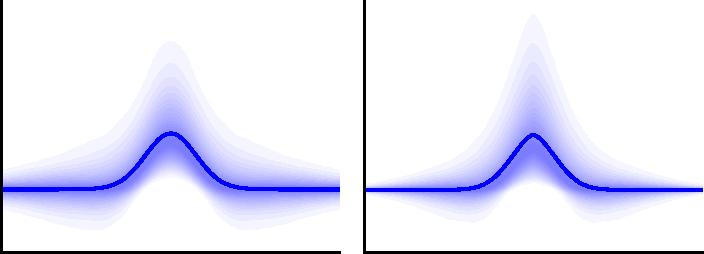
\includegraphics[width=\linewidth, height=3cm]{resources/cropped/prior.pdf}
    \caption{Prior distribution over kernels in the GPCM and CGPCM. Lines correspond to means and gradients indicate marginal variance.}
    \label{fig:prior}
\end{figure}
\begin{figure}[t]
    \centering
    \begin{tabularx}{\linewidth}{>{\centering}X>{\centering}X}
        ~~GPCM & ~~~~~~CGPCM
    \end{tabularx}
    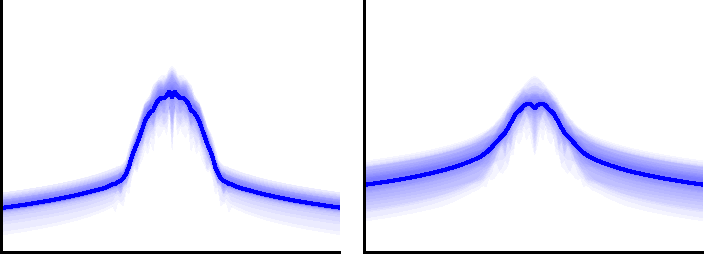
\includegraphics[width=\linewidth, height=3cm]{resources/cropped/prior_psd.pdf}
    \caption{Prior distribution over PSDs in the GPCM and CGPCM. The unit on the $y$ axis is decibel. Lines correspond to means and gradients indicate marginal variance.}
    \label{fig:prior_psd}
\end{figure}

\subsection{Sampling from the CGPCM}
Sampling from the CGPCM is challenging because the integrals in \cref{mod:cgpcm,mod:cgpcm2} depend on the entirety of $h$ and $x$. To resolve this issue, we follow \citet{Tobar:2015:Learning_Stationary} and approximate \cref{eq:kernel} using Bayesian quadrature \cite{Minka:2000:Quadrature_GP} by conditioning on finitely many values $u=(h(t_{u,1}),\ldots,h(t_{u,n_u}))\sim \mathcal{N}(0,K_u)$ of $h$, which induces a  distribution over covariance functions. The mean of this distribution is an accurate approximation for $k_{f\cond h}$ if sufficient conditioning values are used,
\begin{align*}
    k_{f\cond h}(r)
    &\approx \mathbb{E}[k_{f\cond h}(r)\cond u]
    = \int_{0} \mathbb{E}[h(|r| + \tau) h(\tau)\cond u] \id{\tau} \\
    &= \int_0 k_h(|r| + \tau, \tau) \id{\tau} \\
    &\phan{=}+ \mathrm{trace} \left( M^u \int_{0} k_h(t_u, |r|+ \tau)k_h(\tau, t_u^T) \id{\tau} \right)
\end{align*}
where $M^{u}=K_u^{-1}uu^T K_u^{-1}-K_u$. This expression was used to compute the model samples shown in \cref{fig:prior,fig:prior_psd,fig:interpolation}. %Unlike the GPCM, the kernel approximation $\mathbb{E}[k_{f\cond h}(r)\cond u]$ of the CGPCM will not simply be a mixture of Gaussians; it will be a more complicated expression instead.


\subsection{Roughness of Sample Paths}
\label{subsec:roughness}
We now show that the CGCPM can capture both differentiable and nondifferentiable phenomena, the latter in various levels of roughness. In this regard, the model is more flexible than the original GPCM whose sample paths are always differentiable. Let $h$ be a fixed filter that decays to zero at infinity. We claim that $f$'s sample paths are almost surely everywhere differentiable if $h(0)=0$, and almost surely nowhere differentiable if $h(0)\neq 0$. To show this, let $g(r) = \int_0 h(r + \tau) h(\tau) \id{\tau}$ so that
\begin{align*}
    k_{f\cond h}(r) = \! g(|r|) \! = \! g(0) \! + \! g'(0)|r| + \frac{1}{2}g''(0)r^2 + \O(|r|^3).
\end{align*}
Then, according to theorem 2.6 and example 2.3 in section 2.3.1.2 in \cite{Lindgren:2006:Lectures_on_Stationary_Stochastic_Processes}, $f$'s sample paths are almost surely everywhere differentiable if $g'(0)=0$; otherwise, $f$ is not even mean square differentiable, in which case $f$'s sample paths are almost surely nowhere differentiable, according to theorem 5 in \cite{Cambanis:1973:On_Some_Continuity_and_Differentiability}. Finally, it holds that
\begin{align*}
    g'(0)= \int_0 h'(\tau) h(\tau) \id{\tau} = \ll[ h^2(\tau)\rr]_0 - \int_0 h(\tau) h'(\tau) \id{\tau},
\end{align*}
which shows that $g'(0) = -\frac{1}{2} h^2(0)$---we assumed that $h$ decays to zero at infinity. Hence the claim is shown.

In the case that $h(0)\neq 0$, we can locally approximate $f$ by a scaled Wiener process; this scale $\sigma^2$ then quantifies the roughness of the sample paths. Specifically, given that the variance of an increment of a Wiener process is equal the increment's length, we have that
\begin{align*}
    \sigma^2
    &= \lim_{\e \downarrow 0} \frac{\mathbb{V}[f(t+\e)-f(t)]}{\e} \\
    &= \lim_{\e \downarrow 0} \frac{2k_{f\cond h}(0) - 2k_{f\cond h}(\e)}{\e}
    = -2g'(0)
    = h^2(0).
\end{align*}

In summary, the CGPCM models differentiable phenomena if $h(0)=0$ and non-differentiable phenomena if $h(0)\neq 0$. In the latter case $|h(0)|$ quantifies the level of roughness. Performing inference for the filter will therefore automatically infer the differentiability of the underlying process from possibly noisy data.

\Cref{fig:interpolation} shows the filter $h$, the kernel $k_{f\cond h}$, and a sample $f\cond h \sim \mathcal{GP}(0,k_{f\cond h}(t-t'))$ while the filter is interpolated from one that satisfies $h(0)=0$ to one that satisfies $|h(0)|>0$. Note that the sample appears smooth for $h(0)=0$ and becomes rougher as $|h(0)|$ increases.

\begin{figure*}[t]
    \vskip 0.1in
    \centering
    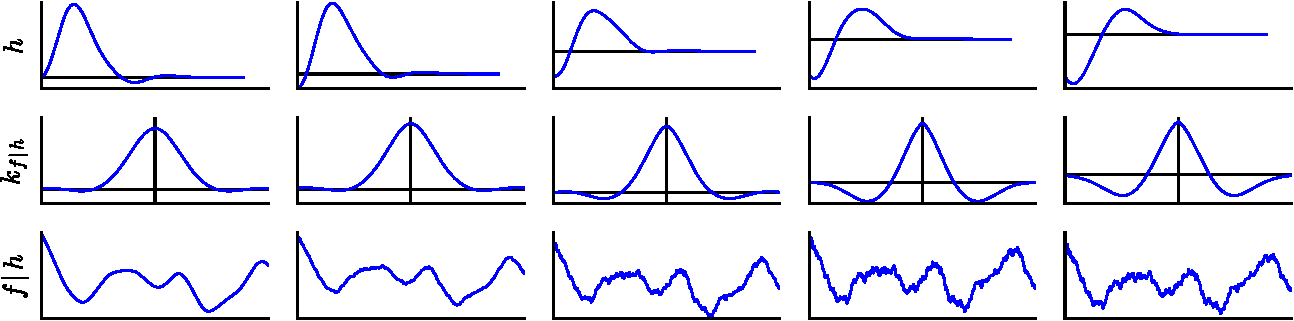
\includegraphics[width=\linewidth]{resources/cropped/interpolation.pdf}
    \caption{Generative process of the CGPCM. Shows the filter $h$, the kernel $k_{f\cond h}$, and a sample $f\cond h \sim \mathcal{GP}(0,k_{f\cond h}(t-t'))$ while the filter is interpolated from one that satisfies $h(0)=0$ to one that satisfies $|h(0)|>0$.}
    \label{fig:interpolation}
    % \vskip -0.2in
\end{figure*}


\section{Inference}
\label{sec:inference}
Let $y(t)\cond \sim \mathcal{N}(f(t),\sigma^2)$ for all $t$ be a noisy version of $f$. Given some observations $e=(y(t_1),\ldots,y(t_n))$ of $y$, we wish to compute $p(f,h,x\cond e)$.

We learn $h$ and $x$ through inducing points \cite{Titsias:2009:Variational_Learning} $u=(h(t_{u,1}),\ldots,h(t_{u,n_u}))\sim \mathcal{N}(0,K_u)$ and $z=(s(t_{z,1}),\ldots,s(t_{z,n_z}))\sim \mathcal{N}(0,K_z)$ for respectively the processes $h$ and $s=T[x]$ where
\begin{align*}
    T[x](t)=\int r(t- \tau)x(\tau) \id{\tau}
\end{align*}
is some interdomain transformation of the white-noise process with filter $r$ \cite{Lazaro-Gredilla:2009:Inter-Domain_Gaussian_Processes_for_Sparse,Alvarez:2010:Efficient_Multioutput_Gaussian_Processes_Through,Tobar:2015:Learning_Stationary}. The inter-domain transformation is necessary because white noise is uncorrelated and so placing inducing points directly in this domain would not be able to capture meaningful structure in the posterior. In choosing $r$, we make sure that $s=T[x]$ has power at the majority of frequencies present in the signal that we aim to model, thereby enabling the inducing variables to capture posterior dependencies in the components of the white noise that pass through the filter and therefore affect the data. We follow \citet{Tobar:2015:Learning_Stationary} and let $r(t)=\exp(-\omega t^2)$, which fits the low frequency components of the posterior.

Let the \textit{mean-field} (MF) approximation $q(f,u,z)=p(f\cond u, z)q(u)q(z)$ of $p(f,u,z\cond e)$ be such that it is closest to $p(f,u,z\cond e)$ in Kullback-Leibler divergence. Contrary to the formulation of \citet{Tobar:2015:Learning_Stationary}, we have analytically integrated out $h$ and $x$ in $p(f\cond u, z)=\int p(f, h, x\cond u, z)\id{h}\id{x}$ prior to performing inference. It is indeed the case that $p(f\cond u, z)$ is intractable, but its first two moments can actually be computed, and only those we need in formulating our inference scheme. Rearranging
\begin{align*}
    &\log p(e) - \KL(q(f,u,z)\|p(f,u,z\cond e)) \\
    &\quad= \ll\la \log \frac{p(e\cond f)\cancel{p(f\cond u, z)}p(u)p(z)}{\cancel{p(f\cond u, z)}q(u)q(z)} \rr\ra_{q(f,u,z)} \\
    &\quad= \underbrace{\la \log p(e\cond f) \ra_{q(f,u,z)}}_{\text{reconstruction cost}} \\
    &\quad\phan{=}- \underbrace{\ll(\ll\la\log\frac{q(u)}{p(u)}\rr\ra_{q(u)} + \ll\la\log\frac{q(z)}{p(z)}\rr\ra_{q(z)}\rr)}_{\text{divergence from prior}} \\
    &\quad=\mathcal{L}[q(u),q(z)]
\end{align*}
shows that we can find $q(u)$ and $q(z)$ through maximising $\mathcal{L}$. Since $\log p(e)\ge\mathcal{L}$, $\mathcal{L}$ is called the \textit{evidence lower bound} (ELBO). Observe that maximisation of $\mathcal{L}$ attempts to explain the data well whilst not diverging too far from the model prior.

To optimise $\mathcal{L}$ with respect to $q(u)$ and $q(z)$ we set their respective variations $\delta \mathcal{L} / \delta q(u)$ and $\delta \mathcal{L} / \delta q(z)$ to zero; then solving for $q(u)$ and $q(z)$ yields
\begin{align}
    q(u) &\propto p(u) \exp \la \log p(e\cond f) \ra_{p(f\cond u,z)q(z)}, \label{eq:qu} \\
    q(z) &\propto p(z) \exp \la \log p(e\cond f) \ra_{p(f\cond u,z)q(u)}, \label{eq:qz}
\end{align}
which are computed in \cref{app:computation_quqz}.
\Cref{app:moments_f} shows that the mean and variance of $p(f\cond u, z)$ are respectively linear and quadratic in both $u$ and $z$; therefore, since $p(e\cond f)$ is Gaussian, we can find a stationary point of $\mathcal{L}$ in which both $q(u)$ and $q(z)$ are Gaussian. Hence, to find $q(u)$ and $q(z)$, we can initialise $q(u)$ and $q(z)$ to some Gaussian and either iterate \cref{eq:qu,eq:qz} or maximise $\mathcal{L}$ directly using gradient-based optimisation. In the latter case we can include any hyperparameter in the optimisation.

One of the new contributions of this work is the finding that we can significantly speed up the optimisation by solving for either $q(u)$ or $q(z)$ analytically. Substituting the optimal form of $q(z)$ back in $\mathcal{L}$ yields
\begin{align}
    &\mathcal{L}^*[q(u)] \nonumber\\
    &\quad=\max_{q(z)} \mathcal{L}[q(u),q(z)]\nonumber\\
    &\quad= \log \int p(z)\exp \la \log p(e\cond f) \ra_{p(f\cond u, z)q(u)} \id{z} \nonumber\\
    &\quad\phan{=}-\ll\la\log\frac{q(u)}{p(u)}\rr\ra_{q(u)},\label{eq:saturated_elbo}
\end{align}
which is computed in \cref{app:saturated_elbo}. We optimise this saturated lower bound $\mathcal{L}^*$ to yield $q(u)$ and then obtain $q(z)$ through \cref{eq:qz}.

Variational mean-field approaches to inference, like the one just presented, are often computationally efficient, but they are known to suffer from certain biases \cite{MacKay:2002:Information_Theory_Learning,Turner:2011:Two_Problems_With_Variational_Expectation,Murphy:2012:Probabilistic_Perspective}. We further refine the MF approximation to alleviate these biases, which is the second major improvement to inference and learning provided by this work.

To this end, let the \textit{structured mean-field} (SMF) approximation $q(f,u,z)=p(f\cond u, z)q(u,z)$ of $p(f,u,z\cond e)$ be such that it that is closest to $p(f,u,z\cond e)$ in Kullback-Leibler divergence. Note that the only assumption underlying the SMF approximation is sufficiency of $u$ and $z$ for respectively $h$ and $s$; hence, the SMF approximation will be close the true posterior in the case that there are sufficiently many $u$ and $z$.

Following a similar argument to the above, we again derive the corresponding ELBO:
\begin{align*}
    &\mathcal{L}[q(u),q(z\cond u)] \\
    &\quad= \la \log p(e\cond f) \ra_{q(f,u,z)}- \ll\la\log\frac{q(u)q(z\cond u)}{p(u)p(z)}\rr\ra_{q(u)q(z\cond u)}.
\end{align*}
Again, setting the variations $\delta \mathcal{L} / \delta q(u)$ and $\delta \mathcal{L} / \delta q(z\cond u)$ to zero and solving for respectively $q(u)$ and $q(z\cond u)$ yields
\begin{align}
    q(u) &\propto p(u) \int p(z) \exp\la\log p(e\cond f)\ra_{p(f\cond u, z)}\id{z}, \label{eq:qu-smf} \\
    q(z\cond u) &\propto p(z)\exp\la \log p(e\cond f)\ra_{p(f\cond u, z)}, \label{eq:qz-smf}
\end{align}
which are computed in \cref{app:computation_quz}.
As opposed to \cref{eq:qu,eq:qz}, \cref{eq:qu-smf,eq:qz-smf} are uncoupled, but $q(u)$'s moments are now intractable. We can, however, evaluate $q(u)$. We therefore use elliptical slice sampling (ESS) \cite{Murray:2010:Elliptical_Slice_Sampling} to sample from $q(u)$ and use these samples to approximate $q(f, u, z)$. To help mixing the Markov chain, we initialise the sampler with the MF approximation.

\section{Experiments}
We test the CGPCM by applying it to synthetic and real-world signals. We show that in certain situations the causality constraint provides an useful inductive bias that leads to better predictions.

% We used TensorFlow \cite{Abadi:2016:TensorFlow_A_System_for_Large-Scale} to implement the CGPCM.\footnote{The implementation can be found at
% % \url{https://github.com/wesselb/cgpcm}.
% --- ---
% } The main issue in implementing the CGPCM is that computation of the matrices in \cref{app:moments_f} requires evaluation of the bivariate normal cumulative density function (BNCDF) \cite{Genz:2004:Numerical_Computation_of_Rectangular_Bivariate}. Unfortunately, the BNCDF is not available in TensorFlow; we therefore we used the implementation of the BNCDF from the R package \texttt{pbivnorm}\footnote{See \url{https://github.com/brentonk/pbivnorm}.} to implement the BNCDF and its gradient in TensorFlow. Moreover, we implementated an algorithm that symbolically solves the integrals in \cref{app:moments_f}; hence we provide no closed-form expression for those integrals.

\subsection{Learning Rough Signals}
In \cref{subsec:roughness} we showed that the CGPCM models both smooth and rough signals, whereas the GPCM models only smooth signals. We perform two experiments that show the significance of this modelling capability.

\begin{figure*}[t]
    \centering
    GPCM
    \begin{tabularx}{\linewidth}{
            >{\centering}>{\hsize=.43\hsize}X  % ??
            >{\centering}>{\hsize=.2\hsize}X
            >{\centering}>{\hsize=.2\hsize}X
            >{\centering}>{\hsize=.2\hsize}X
        }
        $f\cond h$ & $h$ & $k_{f\cond h}$ & PSD of $f\cond h$
    \end{tabularx}
    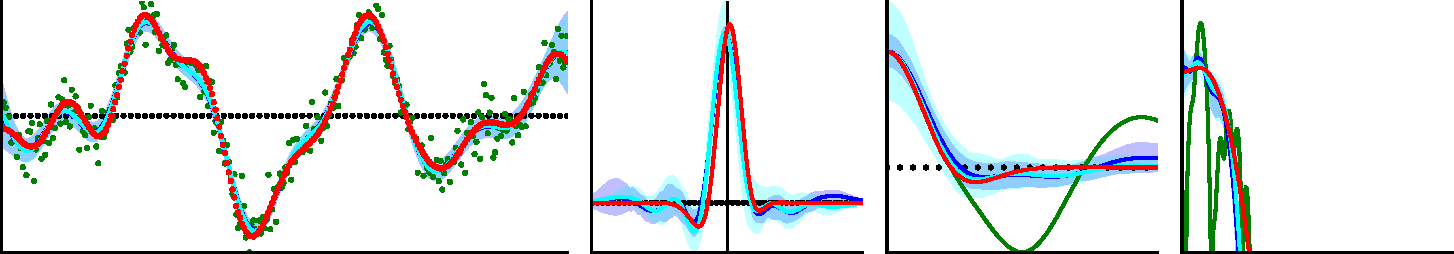
\includegraphics[width=\linewidth, height=3cm]{resources/cropped/learning_known_kernels_acausal_sample_gpcm.pdf}
    CGPCM
    \begin{tabularx}{\linewidth}{
            >{\centering}>{\hsize=.43\hsize}X  % ??
            >{\centering}>{\hsize=.2\hsize}X
            >{\centering}>{\hsize=.2\hsize}X
            >{\centering}>{\hsize=.2\hsize}X
        }
        $f\cond h$ & $h$ & $k_{f\cond h}$ & PSD of $f\cond h$
    \end{tabularx}
    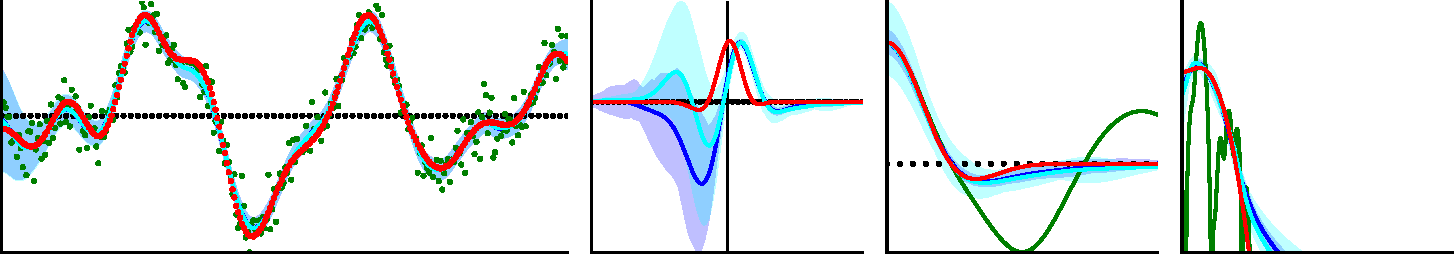
\includegraphics[width=\linewidth, height=3cm]{resources/cropped/learning_known_kernels_acausal_sample_cgpcm.pdf}
    \caption{Predictions of the GPCM and CGPCM after learning a noisy random sample from the GPCM. The learned sample consists of 300 data points. We used 51 evenly-spaced inducing points for $h$ and 80 evenly-spaced inducing points for $x$; inducing points are indicated by black dots in the figure. All parameters were initialised randomly and the procedure from \cref{sec:inference} was followed. All signals are normalised to unity power. {\color{red}Red} denotes truth; {\color{darkgreen}green} denotes observations, the emperical autocorrelation, and the periodogram for respectively the function $f\cond h$, the kernel $k_{f\cond h}$, and the PSD of $f\cond h$; {\color{blue}blue} denotes quantities learned through the MF approximation; and {\color{mycyan}cyan} denotes quantities learned through the SMF approximation. For any learned quantity it holds that lines correspond to means and areas correpond to 95\% central credible regions.}
    \label{fig:toy_acausal_sample}
\end{figure*}

\Cref{fig:toy_acausal_sample} shows the results for fitting the GPCM and CGPCM to a noisy random sample from the GPCM. We make several observations. First, the GPCM and CGPCM appear to both succesfully fit the function $f \cond h$ and the kernel $k_{f\cond h}$. This shows that the CGPCM can indeed learn kernels. Second, the sample from the GPCM appears smooth, which means that the learned filter $h$ for the CGPCM should be nearly zero near zero. A quick inspection of \cref{fig:toy_acausal_sample} verifies that this is indeed the case. Finally, the learned filter $h(t)$ for the CGPCM appears uncertain for $t\le 0$. This a direct consequence of the causality contraint: \cref{eq:model} shows that $f\cond h$ does not depend on $h(t)$ for $t \le 0$.

\begin{figure*}[t]
    \centering
    GPCM
    \begin{tabularx}{\linewidth}{
            >{\centering}>{\hsize=.43\hsize}X  % ??
            >{\centering}>{\hsize=.2\hsize}X
            >{\centering}>{\hsize=.2\hsize}X
            >{\centering}>{\hsize=.2\hsize}X
        }
        $f\cond h$ & $h$ & $k_{f\cond h}$ & PSD of $f\cond h$
    \end{tabularx}
    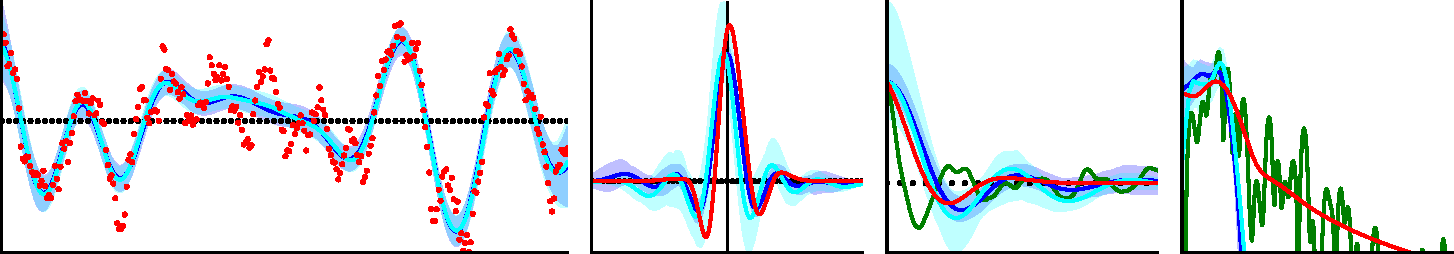
\includegraphics[width=\linewidth, height=3cm]{resources/cropped/learning_known_kernels_causal_sample_gpcm.pdf}
    CGPCM
    \begin{tabularx}{\linewidth}{
            >{\centering}>{\hsize=.43\hsize}X  % ??
            >{\centering}>{\hsize=.2\hsize}X
            >{\centering}>{\hsize=.2\hsize}X
            >{\centering}>{\hsize=.2\hsize}X
        }
        $f\cond h$ & $h$ & $k_{f\cond h}$ & PSD of $f\cond h$
    \end{tabularx}
    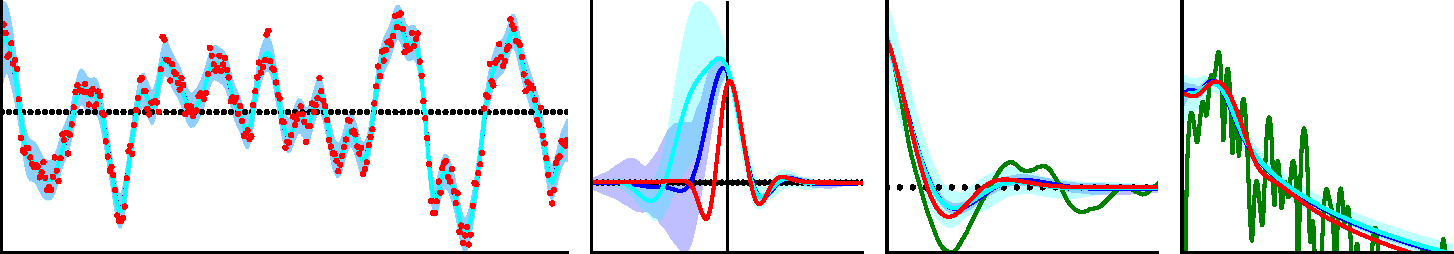
\includegraphics[width=\linewidth, height=3cm]{resources/cropped/learning_known_kernels_causal_sample_cgpcm.pdf}
    \caption{Predictions of the GPCM and CGPCM after learning a noiseless random sample from the CGPCM. The learned sample consists of 300 data points. We used 51 evenly-spaced inducing points for $h$ and 80 evenly-spaced inducing points for $x$; inducing points are indicated by black dots in the figure. All parameters were initialised randomly and the procedure from \cref{sec:inference} was followed. All signals are normalised to unity power. {\color{red}Red} denotes truth; {\color{darkgreen}green} denotes observations, the emperical autocorrelation, and the periodogram for respectively the function $f\cond h$, the kernel $k_{f\cond h}$, and the PSD of $f\cond h$; {\color{blue}blue} denotes quantities learned through the MF approximation; and {\color{mycyan}cyan} denotes quantities learned through the SMF approximation. For any learned quantity it holds that lines correspond to means and areas correpond to 95\% central credible regions.}
    \label{fig:toy_causal_sample}
\end{figure*}

\Cref{fig:toy_causal_sample} shows the results for fitting the GPCM and CGPCM to instead a \textit{noiseless} random sample from the CGPCM. Since the drawn filter $h$ satisfies $|h(0)|>0$, the sample is rough and thus appears noisy. The challenge for the models is to not mistake this sample roughness for observation noise. Observe that the CGPCM fits the filter $h$ and kernel $k_{f \cond h}$ well, whereas GPCM's fit is mediocre. Despite approximately capturing the correlation structure, the GPCM mistakes the sample roughness for observation noise and provides a poor fit of the function $f\cond h$. The CGPCM, on the other hand, correctly recognises the sample roughness and provides an excellent fit of $f \cond h$. This discrepancy is explained by inspecting the fit of the PSD: the GPCM is unable to fit the higher frequencies in the sample, whereas the CGPCM does so succesfully; this is consistent with the priors depicted in \cref{fig:prior_psd}.

The key difference between \cref{fig:toy_acausal_sample,fig:toy_causal_sample} is that in the former noise is added independently, whereas in the latter noise is part of the process dynamics. Therefore \cref{fig:toy_acausal_sample,fig:toy_causal_sample} indicate that the GPCM and CPGCM can both handle independently added noise, but only the CGPCM fits noisy dynamics.

Finally, note that the SMF approximation consistently has better calibrated credible regions compared to the MF approximation. For example, the MF approximation fails to capture the truth in its credible region for the filter $h$, kernel $k_{f\cond h}$, and PSD of $f \cond h$ of the CGPCM in \cref{fig:toy_causal_sample}; in contrast, the SMF approximation does capture the truth.
% \subsection{Speech}
% Coming up.

% \begin{figure*}[t]
%     \centering
%     \begin{tabularx}{\linewidth}{>{\centering}X>{\centering}X}
%         GPCM & CGPCM
%     \end{tabularx}
%     \begin{tabularx}{\linewidth}{>{\centering}X>{\centering}X>{\centering}X>{\centering}X}
%         $k_{f\cond h}$ & PSD of $f\cond h$ & $k_{f\cond h}$ & PSD of $f \cond h$
%     \end{tabularx}
%     % \includegraphics[width=.49\linewidth, height=3cm]{resources/psd_gpcm.pdf}
%     % \includegraphics[width=.49\linewidth, height=3cm]{resources/psd_cgpcm.pdf}
%     \caption{PSD. Here {\color{red}red} denotes truth, {\color{blue}blue} denotes quantities learned through the MF approximation, and {\color{mycyan}cyan} denotes quantities learned through the SMF approximation. All signals are normalised to unity power.}
%     \label{fig:psd}
% \end{figure*}

% Check out \cref{fig:psd}.

\subsection{Head-Related Impulse Response Estimation}
The head-related impulse response (HRIR) describes how sounds entering the ear canal are filtered by the outer ear. The form of the filter depends on the location of the sound source. The filter introduces complex spectral cues into the sounds that are used by the brain to infer source location. We consider the problem of inferring the HRIR from an incoming sound pressure waveform. Suppose that the sound is background noise and can be modelled by white noise. Then assuming a Gaussian process prior over the HRIR we recover the CGPCM exactly; in other words, we can infer the HRIR via inferring the filter $h$ in the CGPCM.

\begin{figure*}[t]
    \centering
    \begin{tabularx}{\linewidth}{>{\centering}X>{\centering}X}
        GPCM & CGPCM
    \end{tabularx}
    \begin{tabularx}{\linewidth}{>{\centering}X>{\centering}X>{\centering}X>{\centering}X}
        $k_{f\cond h}$ & $h$ & $k_{f\cond h}$ & $h$
    \end{tabularx}
    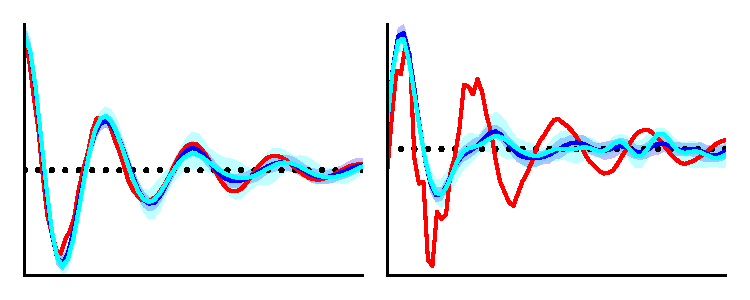
\includegraphics[width=.49\linewidth, height=3cm]{resources/hrtf_gpcm.pdf}
    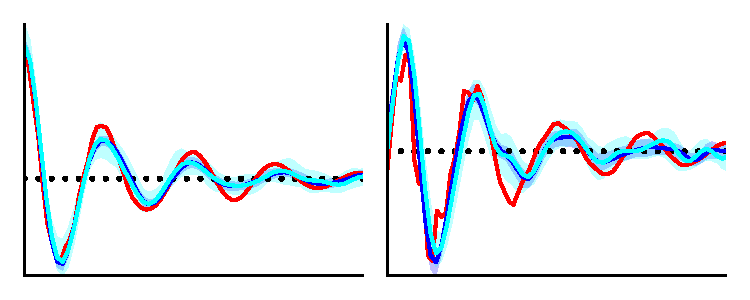
\includegraphics[width=.49\linewidth, height=3cm]{resources/hrtf_cgpcm.pdf}
    \caption{Predictions of the GPCM and CGPCM after learning a HRIR convolved with white noise. The learned sample consists of 500 data points. We used 101 evenly-spaced inducing points for $h$ and 150 evenly-spaced inducing points for $x$; inducing points are indicated by black dots in the figure. All parameters were initialised randomly and the procedure from \cref{sec:inference} was followed. All signals are normalised to unity power. {\color{red}Red} denotes truth, {\color{blue}blue} denotes quantities learned through the MF approximation, and {\color{mycyan}cyan} denotes quantities learned through the SMF approximation. For any learned quantity it holds that lines correspond to means and areas correpond to 95\% central credible regions.}
    \label{fig:hrir}
\end{figure*}

We convolve a HRIR from a KEMAR\footnote{See \url{http://sound.media.mit.edu/resources/KEMAR.html}.} dummy head microphone with white noise to simulate the signal that would have been sensed by the ear. \Cref{fig:hrir} shows the results of fitting the GPCM and CGPCM to the resulting signal. Despite the fact that both models correctly infer the kernel $k_{f \cond h}$, only the CGPCM is able to provide a good prediction for the HRIR. This shows that the inductive bias built in by the causality constraint does in fact help when dealing with causal phenomena.


\section{Discussion}
We have presented the CGPCM as a model of causal, spectrally complex dynamical phenomena. Inference in the CGPCM is performed in a two-step procedure: first a collapsed varational MF approach is used to obtain an initial approximation, and then this approximation is refined through a variational SMF approach combined with ESS. The CGPCM has been tested on synthesised and real-world signals and shows encouraging results. In particular, the CGPCM shows the capability of modelling rough signals without attributing this roughness to observation noise.

Various directions could be explored in future research: First, the model could be extented to multidimensional input and output spaces by following a construction similar to that by \citet{Bruinsma:2016:GGPCM}. Second, the application of more efficient sparse approximation for $h$ and $x$, such as the tree-structured approximation \cite{Bui:2014:Tree-Structured_Gaussian}, would scale the CGPCM to larger data sets. Third, to deal with signals that are band-limited, but not necessarily baseband, the use of an harmonic interdomain transformation \cite{Tobar:2015:Inter-Domain_Inducing} could be explored.
%??? Fourth, in the low noise case, ESS has a hard time exploring $q(u)$; therefore, in that case, afternative sampling algorithms such as Hamiltonian Monte-Carlo \cite{Neal:2012:MCMC_Using_Hamiltonian_Dynamics} could be used.
Finally, using an approach similar to that by \citet{Lazaro-Gredilla:2013:Variational_Inference_for_Mahalanobis_Distance}, Bayesian inference in the hyperparameters could be attempted.

\appendix
\section{Moments of $f\cond u, h$}
\label{app:moments_f}
We solve for $\la f(t) \ra_{p(f\cond u,z)}$ and $\la f(t) f(t') \ra_{p(f\cond u,z)}$. First, we have that
\begin{align*}
    &\la f(t) \ra_{p(f\cond u,z)} \\
    &\quad= \int^t \la h(t - \tau)\ra_{p(f\cond u)} \la x(\tau) \ra_{p(x\cond z)} \id{\tau} \\
    &\quad= u^T K_u^{-1} \underbrace{\int^t k_h(t_u,t-\tau) k_{xs}(\tau, t_z^T) \id{ \tau}}_{A^{hx}(t)=A^{(xh)T}(t)} K_z^{-1} z.
\end{align*}
Second, it holds that

\begin{align*}
    &\la f(t) f(t') \ra_{p(f\cond u,z)} \\
    &\quad= \int^t\!\!\!\!\int^{t'} \la h(t- \tau) h(t' - \tau')\ra_{p(h\cond u)} \\
    &\quad\phan{=\int^t\!\!\!\!\int^{t'}} \la x(\tau) x(\tau') \ra_{p(x\cond z)}\id{\tau'}\id{\tau} \\
    &\quad= \int^t\!\!\!\!\int^{t'} ( k_h(t- \tau,t' - \tau') \\
    &\quad\phan{=\int^t\!\!\!\!\int^{t'} (}+ k_h(t- \tau, t_u^T) M^u k_h(t_u, t' - \tau')) \\
    &\quad\phan{=\int^t\!\!\!\!\int^{t'}}( k_x(\tau,\tau') + k_{xs}(\tau, t_z^T) M^z k_{sx}(t_z, \tau')) \id{\tau'}\id{\tau} \\
    &\quad= a(t,t') + \tr M^u A^{h}(t,t') + \tr M^z A^{x}(t,t') \\
    &\quad\phan{=} + \tr M^u A^{hx}(t) M^z A^{xh}(t')
\end{align*}
where $M^u=K_u^{-1}uu^T K_u^{-1}-K_u^{-1}$, $M^z=K_z^{-1}zz^TK_z^{-1}-K_z^{-1}$, and
\begin{align*}
    a(t,t')&=\int^t\!\!\!\!\int^{t'} k_h(t- \tau,t' - \tau') k_x(\tau,\tau') \id{\tau'}\id{\tau} \\
    &=\int^{t \land t'} k_h(t- \tau,t' - \tau)\id{\tau}, \\
    A^{h}(t,t')&=\int^t\!\!\!\!\int^{t'} k_h(t_{u}, t' - \tau') k_x(\tau,\tau') \\
    &\phan{=\int^t\!\!\!\!\int^{t'}}\, k_h(t- \tau, t_{u}^T) \id{\tau'}\id{\tau}\\
    &=\int^{t \land t'} k_h(t_{u}, t' - \tau)k_h(t- \tau, t_{u}^T) \id{\tau}  \\
    A^{x}(t,t')&=\int^t\!\!\!\!\int^{t'} k_{sx}(t_z, \tau') k_h(t- \tau,t'-\tau') \\
    &\phan{=\int^t\!\!\!\!\int^{t'}}\, k_{xs}(\tau, t_z^T) \id{\tau'}\id{\tau}.
\end{align*}
Rearranging, we arrive at $\la f(t) \ra = u^T  A^{hx}(t) z$ and
\begin{align*}
    &\la f(t) f(t') \ra - \la f(t) \ra \la f(t') \ra \\
    &\quad = b(t,t') + u^T B^{h}(t,t') u + z^T B^{x}(t,t') z
\end{align*}
where the expectation is over $p(f\cond K_u^{-1} u, K_z^{-1} z)$ and
\begin{align*}
    b(t,t) &= a(t,t') - \tr K_u^{-1} A^{h}(t,t') - \tr K_z^{-1}A^{x}(t,t') \\
    &\phan{=} + \tr K_u^{-1}A^{hx}(t)K_z^{-1}A^{xh}(t'), \\
    B^{h}(t,t') &= A^{h}(t,t') - A^{hx}(t)K_z^{-1} A^{xh}(t'), \\
    B^{x}(t,t') &= A^{x}(t,t') - A^{xh}(t)K_u^{-1} A^{hx}(t').
\end{align*}
Finally, we denote $a(t)=a(t,t)$ and do so for $A^h$, $A^x$, $A^{hx}$, $b$, $B^h$, and $B^x$ as well.

% \subsection{Causal Interdomain Transformation}
% In the case of the causal interdomain transformation, $A^{hx}$ and $A^x$ reduce to
% \begin{align*}
%    A^{hx}(t) &=\int^{t\land t_z^T} k_h(t_u,t-\tau) k_{xs}(\tau, t_z^T) \id{ \tau}, \\
%    A^{x}(t,t')&=\int^{t \land t_z}\!\!\!\!\int^{t'\land t_z^T} k_{sx}(t_z, \tau') k_h(t- \tau,t'-\tau') \\
%     &\phan{=\int^{t \land t_z}\!\!\!\!\int^{t'\land t_z^T}}\, k_{xs}(\tau, t_z^T) \id{\tau'}\id{\tau}.
% \end{align*}

\section{MF Approximation: Computation of $q(u)$ and $q(z)$}
\label{app:computation_quqz}
Following \cref{app:moments_f}, we have that
\begin{align*}
    &\la \log p(e\cond f) \ra_{p(f\cond K_u^{-1} u, K_z^{-1} z)} \\
    &\quad= -\frac{n}{2}\log 2 \pi \sigma^2 - \frac{1}{2 \sigma^2} \la e^{2}(t) - 2 \sigma_f u^T A^{hx}(t) e(t) z\\
    &\quad\phan{=}  + \sigma_f^2 ( b(t) + u^T B^{h}(t) u+ z^T B^{x}(t) z \\
    &\quad\phan{=}  + (u^T A^{hx}(t) z)^2 ) \ra_t
\end{align*}
where $\la\,\cdot\,\ra_t$ denotes summation with respect to $t$ over $t_1,\ldots,t_n$.
It follows that
\begin{align*}
    &\log p(K_u^{-1} u)  + \la \log p(e\cond f) \ra_{p(f\cond K_z^{-1}z, K_u^{-1}u)q(K_z^{-1}z)} \\
    &\quad= -\frac{1}{2}u^T\ll(K_u + \frac{\sigma_f^2}{\sigma^2} \la B^{h}(t) \rr.\\[-3\jot]
    &\quad\phan{= -\frac{1}{2}u^T}
        \underbrace{
            \phan{\ll(K_u + \frac{\sigma_f^2}{\sigma^2} \la \rr. } \!\!\!\!\!
            \ll. \vphantom{\frac{\sigma_f^2}{\sigma^2} }
                 + A^{hx}(t)  z z^T A^{xh}(t) \ra_{t,q(K_z^{-1} z)}
            \rr)
        }_{\Sigma_u^{-1}}u \\
    &\quad\phan{=}+ u^T \underbrace{\frac{\sigma_f}{\sigma^2}\la e(t) A^{hx}(t) z\ra_{t,q(K_z^{-1}z)}}_{\Sigma_u^{-1} \mu_u} \\
    &\quad\phan{=}  + \ll(\vphantom{\frac{\sigma_f^2}{2 \sigma^2}} {-\frac{n}{2}}\log 2 \pi \sigma^2-\frac{1}{2}\log|2 \pi K_u^{-1}|  \rr. \\
    &\quad\phan{=+}\underbrace{\phan{ \ll(\vphantom{\frac{\sigma_f^2}{2 \sigma^2}}\rr.}- \frac{\la e^2(t)\ra_t}{2 \sigma^2} - \ll.\frac{\sigma_f^2}{2 \sigma^2}\la b(t) - z^T B^{x}(t) z\ra_{t,q(K_z^{-1}z)}\rr)}_{\text{constant independent of $u$}} \\
    &\quad= \log \underbrace{\mathcal{N}(u; \mu_u, \Sigma_u)}_{q(K_u^{-1}u)}+ \frac{1}{2}\log|2 \pi \Sigma_u| \\
    &\quad\phan{=}+ \frac{1}{2}\mu_u^T \Sigma_u^{-1}\mu_u  + \text{constant independent of $u$}
\end{align*}
and $q(z)$ is derived similarly.

\section{MF Approximation: Saturated ELBO}
\label{app:saturated_elbo}
Following \cref{eq:saturated_elbo} and \cref{app:computation_quqz}, we have that
\begin{align*}
    &\mathcal{L}^*[q(K_u^{-1} u)] \\
    &\quad = - \frac{n}{2}\log 2 \pi \sigma^2 + \frac{1}{2}\log|K_z^{-1}||\Sigma_z| + \frac{1}{2}\mu_z^T \Sigma_z^{-1}\mu_z  \\
    &\quad \phan{=} - \frac{\la e^2(t)\ra_t}{2 \sigma^2}- \frac{\sigma_f^2}{2 \sigma^2}\la b(t) +  u^T B^{h}(t) u \ra_{t,q(K_u^{-1}u)} \\
    &\quad \phan{=}  + \ll\la \log \frac{p(K_u^{-1}u)}{q(K_u^{-1}u)} \rr\ra_{q(K_u^{-1}u)}.
\end{align*}

\section{SMF Approximation: Computation of $q(u)$ and $q(z\cond u)$}
\label{app:computation_quz}
The mean and variance of $q(z\cond u)$ are similar to that of $q(z)$ in \cref{app:computation_quqz} with only the difference being that the expectation with respect to $q(u)$ is omitted.

To compute $q(u)$, we again follow \cref{app:computation_quqz} and have that
\begin{align*}
    \Sigma &= K_z + \frac{\sigma_f^2}{\sigma^2} \la B^x(t) + A^{xh}(t) u u^TA^{hx}(t) \ra_t, \\
    \mu &= \frac{\sigma_f}{\sigma^2}\la e(t) A^{xh}(t)u\ra_{t}, \\
    \log q(K_u^{-1} u) &= \log p(K_u^{-1} u)- \frac{n}{2}\log 2 \pi \sigma^2 -\frac{1}{2}\log|K_z||\Sigma|\\
    &\phan{=}+ \frac{1}{2}\mu^T \Sigma^{-1} \mu- \frac{\la e^2(t)\ra_t}{2 \sigma^2} \\
    &\phan{=}  - \frac{\sigma_f^2}{2 \sigma^2} \la b(t) + u^T B^h(t)u \ra_t.
\end{align*}



\bibliography{bibliography}
\bibliographystyle{icml2017}


% \section{Remarks}
% For the GPCM it holds that
% \begin{align*}
%     \hat{k}_{f\cond h}(\omega) = \int f(t)\exp(- i \omega t)\id{t}=|\hat{h}(\omega)|^2,
% \end{align*}
% whereas for the CGCPM it holds that
% \begin{align*}
%     \hat{k}_{f\cond h}(\omega)
%     &= \frac{1}{4}\ll|\ll(\pi \delta(\omega) -i \frac{1}{\pi \omega}\rr)\ast\hat{h}(\omega)\rr|^2 \\
%     &= \frac{1}{4}\ll|\pi h(\omega) - i (\mathcal{H}\hat{h})(\omega)\rr|^2
% \end{align*}
% where $\mathcal{H}$ is the Hilbert transform. Can this be interpreted?


\end{document}

